% ---- Figure 1 palette ----
\definecolor{bodygray}{RGB}{92,100,112}
\definecolor{faint}{RGB}{158,165,176}
\definecolor{c1line}{RGB}{201,148,74}
\definecolor{c1deep}{RGB}{146,98,36}
\definecolor{c1soft}{RGB}{243,224,192}
\definecolor{c2line}{RGB}{86,131,184}
\definecolor{c2deep}{RGB}{40,76,124}
\definecolor{c2soft}{RGB}{206,223,244}
\definecolor{c3line}{RGB}{62,150,110}
\definecolor{c3deep}{RGB}{22,96,62}
\definecolor{c3soft}{RGB}{198,232,212}


\usetikzlibrary{arrows.meta,backgrounds,calc,positioning,decorations.pathmorphing}
\begin{figure*}[t]
\centering
\resizebox{\textwidth}{!}{%
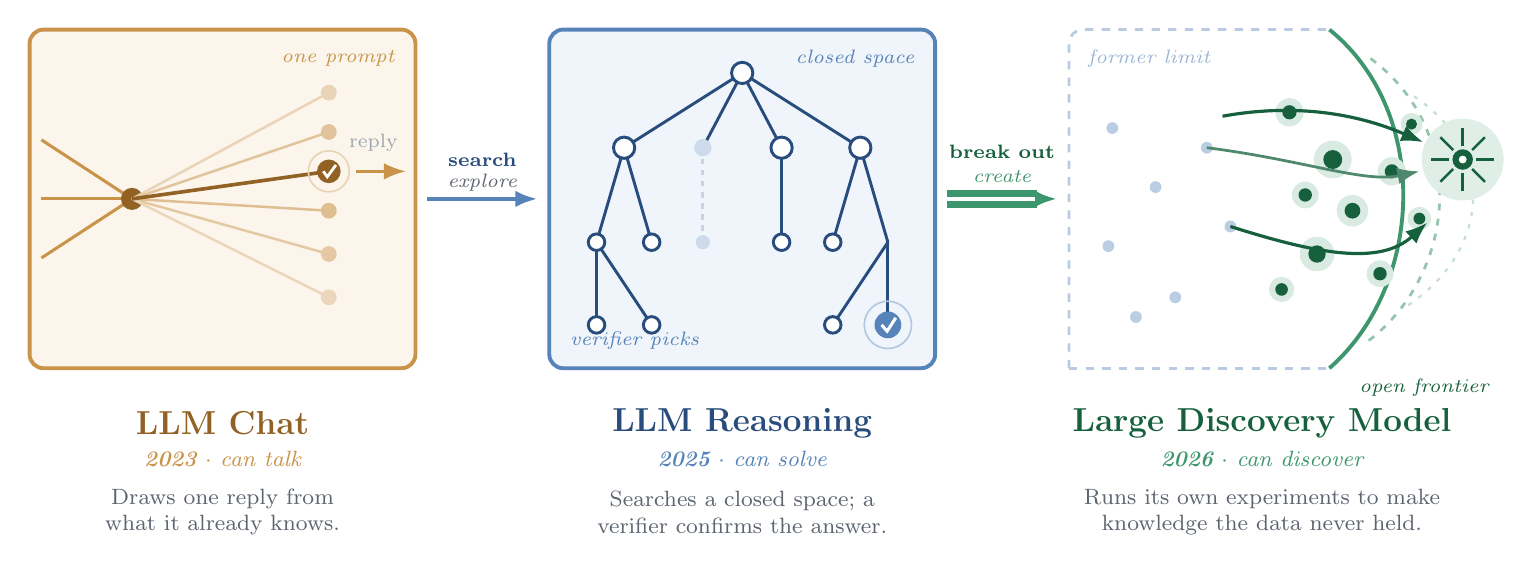
\begin{tikzpicture}[
    >={Latex[length=2.8mm]},
    font=\small,
]

\def\S{6.6}          % stage spacing
\def\HW{2.45}        % panel half-width
\def\HH{2.15}        % panel half-height
\coordinate (P1) at (0,0);
\coordinate (P2) at (\S,0);
\coordinate (P3) at (2*\S,0);

% ============ STAGE 1 -- CHAT ============
\begin{scope}[shift={(P1)}]
  \draw[c1line,line width=1.4pt,rounded corners=5pt,fill=c1soft!32]
        (-\HW,-\HH) rectangle (\HW,\HH);
  \node[font=\scriptsize\itshape,text=c1line,anchor=north east] at (\HW-0.14,\HH-0.14)
        {one prompt};
  \coordinate (src) at (-1.15,0);
  \draw[c1line,line width=1.1pt] (-\HW+0.15,0.75) -- (src);
  \draw[c1line,line width=1.1pt] (-\HW+0.15,-0.75) -- (src);
  \draw[c1line,line width=1.1pt] (-\HW+0.15,0) -- (src);
  \fill[c1deep] (src) circle (0.14);
  \foreach \py/\op in {1.35/40, 0.85/55, 0.35/70, -0.15/60, -0.7/50, -1.25/38}{
     \draw[c1line!\op,line width=0.9pt] (src) -- (1.35,\py);
     \fill[c1line!\op] (1.35,\py) circle (0.10);
  }
  \draw[c1deep,line width=1.3pt] (src) -- (1.35,0.35);
  \draw[c1line!40,line width=0.6pt] (1.35,0.35) circle (0.26);
  \fill[c1deep] (1.35,0.35) circle (0.15);
  \draw[white,line width=1pt] (1.28,0.35)--(1.33,0.28)--(1.44,0.43);
  \draw[->,c1line,line width=1.1pt] (1.7,0.35) -- (\HW-0.12,0.35);
  \node[font=\scriptsize,text=faint,anchor=east] at (\HW-0.1,0.72) {reply};
\end{scope}

% ============ STAGE 2 -- REASONING ============
\begin{scope}[shift={(P2)}]
  \draw[c2line,line width=1.4pt,rounded corners=5pt,fill=c2soft!30]
        (-\HW,-\HH) rectangle (\HW,\HH);
  \node[font=\scriptsize\itshape,text=c2line,anchor=north east] at (\HW-0.14,\HH-0.14)
        {closed space};
  \begin{scope}[c2deep,line width=1.05pt]
    \coordinate (rt) at (0,1.6);
    \coordinate (a) at (-1.5,0.65);
    \coordinate (b) at (-0.5,0.65);
    \coordinate (c) at (0.5,0.65);
    \coordinate (d) at (1.5,0.65);
    \coordinate (a1) at (-1.85,-0.55);
    \coordinate (a2) at (-1.15,-0.55);
    \coordinate (b1) at (-0.5,-0.55);
    \coordinate (c1n) at (0.5,-0.55);
    \coordinate (d1) at (1.15,-0.55);
    \coordinate (d2) at (1.85,-0.55);
    \coordinate (aa) at (-1.85,-1.6);
    \coordinate (ab) at (-1.15,-1.6);
    \coordinate (dd) at (1.15,-1.6);
    \coordinate (de) at (1.85,-1.6);
    \draw (rt)--(a); \draw (rt)--(b); \draw (rt)--(c); \draw (rt)--(d);
    \draw (a)--(a1); \draw (a)--(a2);
    \draw[c2line!35,dash pattern=on 2pt off 2pt] (b)--(b1);
    \draw (c)--(c1n);
    \draw (d)--(d1); \draw (d)--(d2);
    \draw (a1)--(aa); \draw (a1)--(ab);
    \draw (d2)--(dd); \draw (d2)--(de);
    \foreach \p in {rt,a,c,d}{ \fill[white,draw=c2deep] (\p) circle (0.135); }
    \fill[c2line!30] (b) circle (0.11);
    \fill[c2line!30] (b1) circle (0.09);
    \foreach \p in {a1,a2,c1n,d1,aa,ab,dd}{ \fill[white,draw=c2deep] (\p) circle (0.105); }
    \draw[c2line!45,line width=0.6pt] (de) circle (0.30);
    \fill[c2line] (de) circle (0.17);
    \draw[white,line width=1.1pt] ($(de)+(-0.08,0)$)--($(de)+(-0.01,-0.08)$)--($(de)+(0.10,0.09)$);
  \end{scope}
  \node[font=\scriptsize\itshape,text=c2line,anchor=south west] at (-\HW+0.14,-\HH+0.12)
        {verifier picks $\checkmark$};
\end{scope}

% ============ STAGE 3 -- DISCOVERY ============
\begin{scope}[shift={(P3)}]
  \draw[c2line!42,line width=1pt,rounded corners=5pt,dash pattern=on 3pt off 3pt]
        (-\HW,-\HH) -- (-\HW,\HH) -- (\HW*0.35,\HH);
  \draw[c2line!42,line width=1pt,rounded corners=5pt,dash pattern=on 3pt off 3pt]
        (-\HW,-\HH) -- (\HW*0.35,-\HH);
  \node[font=\scriptsize\itshape,text=c2line!60,anchor=north west] at (-\HW+0.12,\HH-0.14)
        {former limit};
  \foreach \px/\py in {-1.9/0.9,-1.35/0.15,-1.95/-0.6,-1.1/-1.25,-0.7/0.65,-1.6/-1.5,-0.4/-0.35}{
     \fill[c2line!40] (\px,\py) circle (0.075);
  }
  \draw[c3line,line width=1.4pt]
        (\HW*0.35,-\HH) .. controls (\HW*0.35+1.2,-1.1) and (\HW*0.35+1.3,1.1) .. (\HW*0.35,\HH);
  \draw[c3line!55,line width=1pt,dash pattern=on 2.5pt off 3pt]
        (\HW*0.35+0.5,-\HH+0.35) .. controls (\HW*0.35+1.65,-0.9) and (\HW*0.35+1.75,0.9) .. (\HW*0.35+0.5,\HH-0.35);
  \draw[c3line!30,line width=0.8pt,dash pattern=on 1.5pt off 3pt]
        (\HW*0.35+1.0,-\HH+0.8) .. controls (\HW*0.35+2.05,-0.65) and (\HW*0.35+2.15,0.65) .. (\HW*0.35+1.0,\HH-0.8);
  \foreach \px/\py/\s in {0.35/1.1/0.09, 0.9/0.5/0.12, 1.15/-0.15/0.10, 0.7/-0.7/0.11,
                          1.65/0.35/0.09, 1.5/-0.95/0.085, 0.25/-1.15/0.08, 2.0/-0.25/0.075,
                          0.55/0.05/0.085, 1.9/0.95/0.07}{
     \fill[c3line!20] (\px,\py) circle (\s*2);
     \fill[c3deep] (\px,\py) circle (\s);
  }
  \begin{scope}[shift={(2.55,0.5)}]
     \fill[c3line!16] (0,0) circle (0.52);
     \foreach \ang in {0,45,90,135,180,225,270,315}{
        \draw[c3deep,line width=0.9pt] (\ang:0.17) -- (\ang:0.40); }
     \fill[c3deep] (0,0) circle (0.13);
     \fill[white] (0,0) circle (0.05);
  \end{scope}
  \draw[->,c3deep,line width=1.15pt] (-0.5,1.05) .. controls (0.6,1.25) and (1.4,1.0) .. (2.05,0.72);
  \draw[->,c3deep,line width=1.15pt] (-0.4,-0.35) .. controls (0.7,-0.7) and (1.5,-0.85) .. (2.1,-0.3);
  \draw[->,c3deep!75,line width=1pt] (-0.7,0.65) .. controls (0.5,0.5) and (1.3,0.2) .. (2.0,0.35);
  \node[font=\scriptsize\itshape,text=c3deep,anchor=north] at (\HW*0.35+1.2,-\HH-0.02)
        {open frontier};
\end{scope}

% ============ CONNECTORS ============
% P1 -> P2
\coordinate (a0) at ($(P1)+(\HW+0.15,0)$);
\coordinate (a1c) at ($(P2)+(-\HW-0.15,0)$);
\draw[->,line width=1.5pt,c2line] (a0) -- (a1c);
\coordinate (gapA) at ($(a0)!0.5!(a1c)$);
\node[font=\bfseries\scriptsize,text=c2deep,align=center,text width=1.55cm]
      at ($(gapA)+(0,0.5)$) {search};
\node[font=\itshape\scriptsize,text=bodygray,align=center,text width=1.55cm]
      at ($(gapA)+(0,0.2)$) {explore};

% P2 -> P3
\coordinate (b0) at ($(P2)+(\HW+0.15,0)$);
\coordinate (b1c) at ($(P3)+(-\HW-0.15,0)$);
\draw[->,line width=2.4pt,c3line,double,double distance=1.5pt] (b0) -- (b1c);
\coordinate (gapB) at ($(b0)!0.5!(b1c)$);
\node[font=\bfseries\scriptsize,text=c3deep,align=center,text width=1.65cm]
      at ($(gapB)+(0,0.6)$) {break out};
\node[font=\itshape\scriptsize,text=c3line,align=center,text width=1.65cm]
      at ($(gapB)+(0,0.28)$) {create};

% ============ LABELS ============
\node[font=\bfseries\large,text=c1deep] at ($(P1)+(0,-2.85)$) {LLM Chat};
\node[font=\itshape\footnotesize,text=c1line] at ($(P1)+(0,-3.3)$) {\textbf{2023} $\cdot$ can talk};
\node[text=bodygray,font=\footnotesize,align=center,text width=4.1cm]
      at ($(P1)+(0,-3.98)$) {Draws one reply from what it already knows.};

\node[font=\bfseries\large,text=c2deep] at ($(P2)+(0,-2.85)$) {LLM Reasoning};
\node[font=\itshape\footnotesize,text=c2line] at ($(P2)+(0,-3.3)$) {\textbf{2025} $\cdot$ can solve};
\node[text=bodygray,font=\footnotesize,align=center,text width=4.6cm]
      at ($(P2)+(0,-3.98)$) {Searches a closed space; a verifier confirms the answer.};

\node[font=\bfseries\large,text=c3deep] at ($(P3)+(0,-2.85)$) {Large Discovery Model};
\node[font=\itshape\footnotesize,text=c3line] at ($(P3)+(0,-3.3)$) {\textbf{2026} $\cdot$ can discover};
\node[text=bodygray,font=\footnotesize,align=center,text width=5cm]
      at ($(P3)+(0,-3.98)$) {Runs its own experiments to make knowledge the data never held.};

\end{tikzpicture}%
}
\caption{\textbf{From generating to discovering.} Three stages of large-model capability.
\emph{LLM chat} draws a single reply from a fixed prior, where the model returns one sample
per prompt. \emph{LLM reasoning} searches a closed space of candidate solutions and keeps the
leaf a cheap verifier confirms, where the reachable set is bounded and known in advance.
\emph{Large discovery models} break past that boundary, designing their own experiments to
create points outside the prior data, where the search frontier stays open and each result
reshapes what can be reached next.}
\label{fig:evolution}
\end{figure*}